The response amplitude operator is given by
\[
    \frac{\hat{\xi}_2}{A} = \frac{X_2}{c_{22} - \omega^2 (m + m_{22}) + i \omega r_{22}},
\]
yielding a condition for which we the hydrostatic forces balancing the inertial forces, namely
\[
    {\omega_n}^2 = \frac{\sfrac{\gravity}{D}}{1 + \frac{m_{22}}{\varrho D L}}.
\]
\begin{Figure}
    \centering
    \captionsetup{type = figure}
    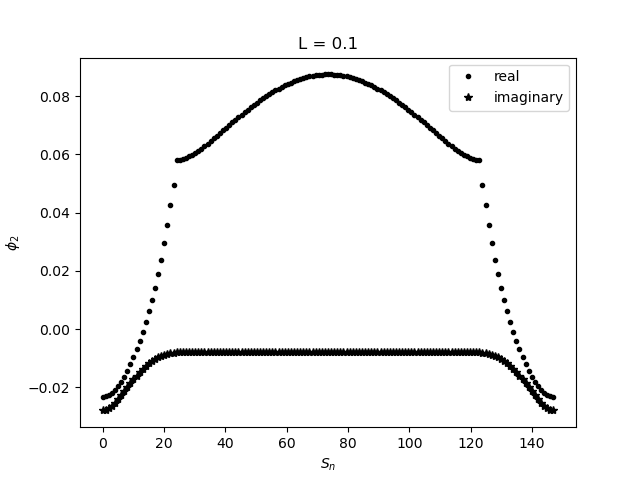
\includegraphics[width = \textwidth]{heave_Lp1_D1_kD1p2.png}
    \caption{Heave for $\sfrac{L}{D} = 0.1$.}
\end{Figure}
\begin{Figure}
    \centering
    \captionsetup{type = figure}
    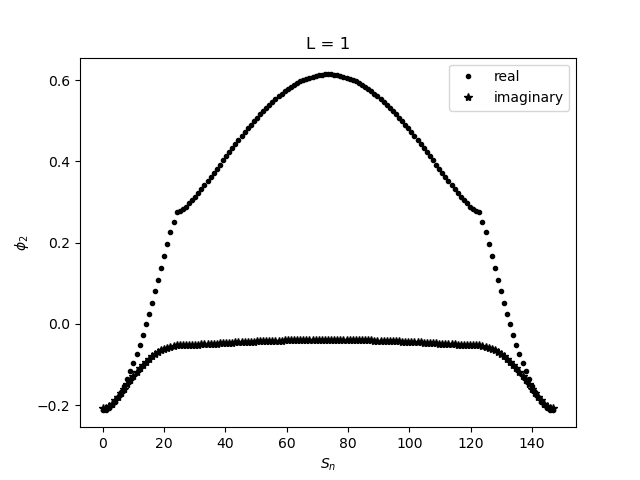
\includegraphics[width = \textwidth]{heave_L1_D1_kD1p2.png}
    \caption{Heave for $\sfrac{L}{D} = 1$.}
\end{Figure}
\begin{Figure}
    \centering
    \captionsetup{type = figure}
    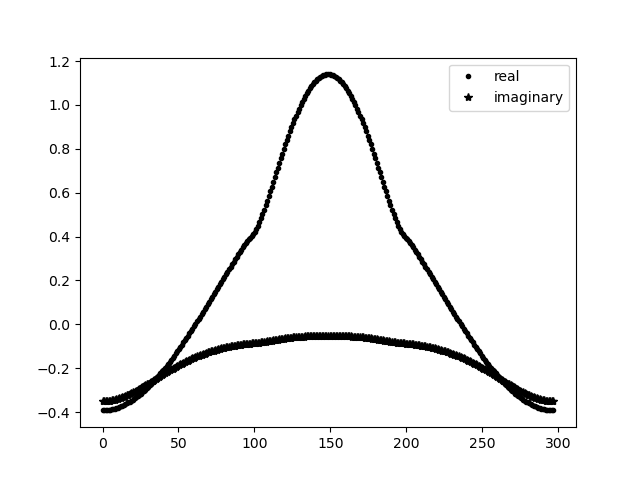
\includegraphics[width = \textwidth]{heave_L2_D1_kD1p2.png}
    \caption{Heave for $\sfrac{L}{D} = 2$.}
\end{Figure}
\begin{Figure}
    \centering
    \captionsetup{type = figure}
    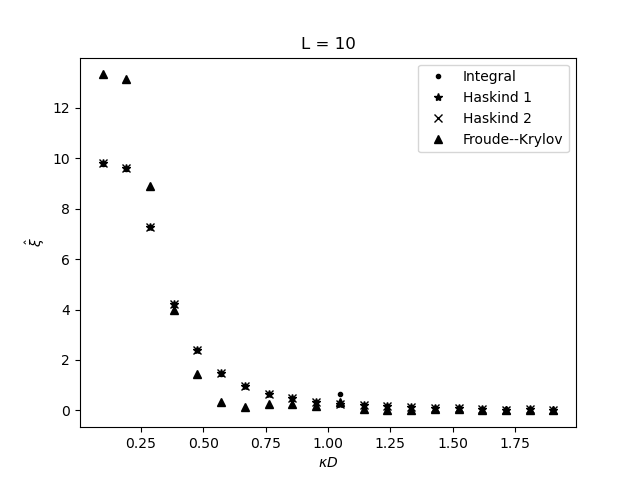
\includegraphics[width = \textwidth]{heave_L10_D1_kD1p2.png}
    \caption{Heave for $\sfrac{L}{D} = 10$.}
\end{Figure}